\section{Auswahlkriterien zu IT-Produkten allgemein unterscheiden}
\subsection{Qualität und Leistungsfähigkeit von IT-Systemen und IT-Services beschreiben}
    \begin{subindent}
        Qualitätsniveau und Qualitätsmanagement werden in der modernen IT immer wichtiger.
        Daher erhöht sich der Anspruch an diese Aspekte innerhalb von Unternehmen stetig. Diese Ansprüche umfassen die in der folgenden Begriffserklärung gelisteten Punkte.
    \end{subindent}

    \begin{tcolorbox}[width=13cm, center, title=Qualitätsbegriff, coltitle=white, colframe=white!20!blue, colback=white!80!blue]
        \begin{enumerate}[itemsep=0.01em, parsep=0.3em]
            \item Beschaffenheit, Merkmal, Eigenschaft, Zustand
            \item Güte aller Eigenschaften eines Objektes, Systems oder Prozesses
            \item Zweckangemessenheit eines Produktes (Produktqualität), einer Dienstleistung (Servicequalität) oder eines Prozesses (Prozessqualität)
        \end{enumerate}
    \end{tcolorbox}

    \begin{subindent}
        Weitere Mängelarten, Mängel und nicht erfüllte Anforderungen, die im Bundesgesetzbuch festgehalten sind:
    \end{subindent}

    \begin{itemize}[leftmargin=2.5cm, topsep=0.3em, itemsep=0.1em, parsep=0.5em]
        \item Sach- und Rechstmangel (§433-435 BGB)
        \item Mangelausschluss (§434, 442 BGB)
        \item Leistungsausschluss (§275 BGB)
    \end{itemize}

    \begin{subindent}
        Bei digitalen Produkten gelten für Unternehmen gegenüber Verbrauchern zusätzliche Regelungen (§327 BGB). \\
        Standards, Normen und Marken:
    \end{subindent}

    \begin{tcolorbox}[width=11cm, center, title=Normen, coltitle=white, colframe=orange, colback=white!60!orange]
        Technische Vorgaben die von Organisationen festgelegt werden. Werden in z.B. Verträgen oder Gesetzen genannt und erhalten dadurch Verbindlichkeit.
        In Gesetzen und Verordnungen ersetzen sie rechtliche Detailregelungen.
    \end{tcolorbox}

    \begin{tcolorbox}[width=10cm, center, title=Abkürzungen, coltitle=white, colframe=white!20!blue, colback=white!80!blue]
        \begin{itemize}[itemsep=0.01em, parsep=0.3em]
            \item[DIN -] Deutsches Institut für Normung
            \item[ISO -] Internationale Organisation für Normung
            \item[IEC -] Internationale Elektrotechnische Normung
            \item[EN -] Normen Europäischer Komitees 
        \end{itemize}
    \end{tcolorbox}

    \begin{subindent}
        \begin{itemize}[leftmargin=2.5cm, topsep=0.3em, itemsep=0.1em, parsep=0.5em]
            \item \textbf{Zertifizierungen:} \\ Prüfdokumente, ausgestellt von anerkannten Zertifizierungsstellen
            \item \textbf{Formfaktoren:} \\ Konstruktionsvorgaben für Größen, Formen und Anschlüsse für Hardware im Markte
            \item \textbf{Marken:} \\ Schutzzeichen, die Unternehmen beim Patent- und Markenamt erlangen können   
        \end{itemize}
    \end{subindent}

    \begin{figure}[ht]
        \centering
        \includegraphics[width=0.7\textwidth]{./images/2.3.1_qualitätskriterien.png}
        \caption{Qualitätskriterien}\label{fig:Qualitätskriterien}
    \end{figure}

\newpage
\subsection{Umweltschutz und Green-IT als wichtige IT-Ziele darstellen}
    %TODO change tcolorboxes to green (cus green it)
    \begin{figure}[ht]
        \centering
        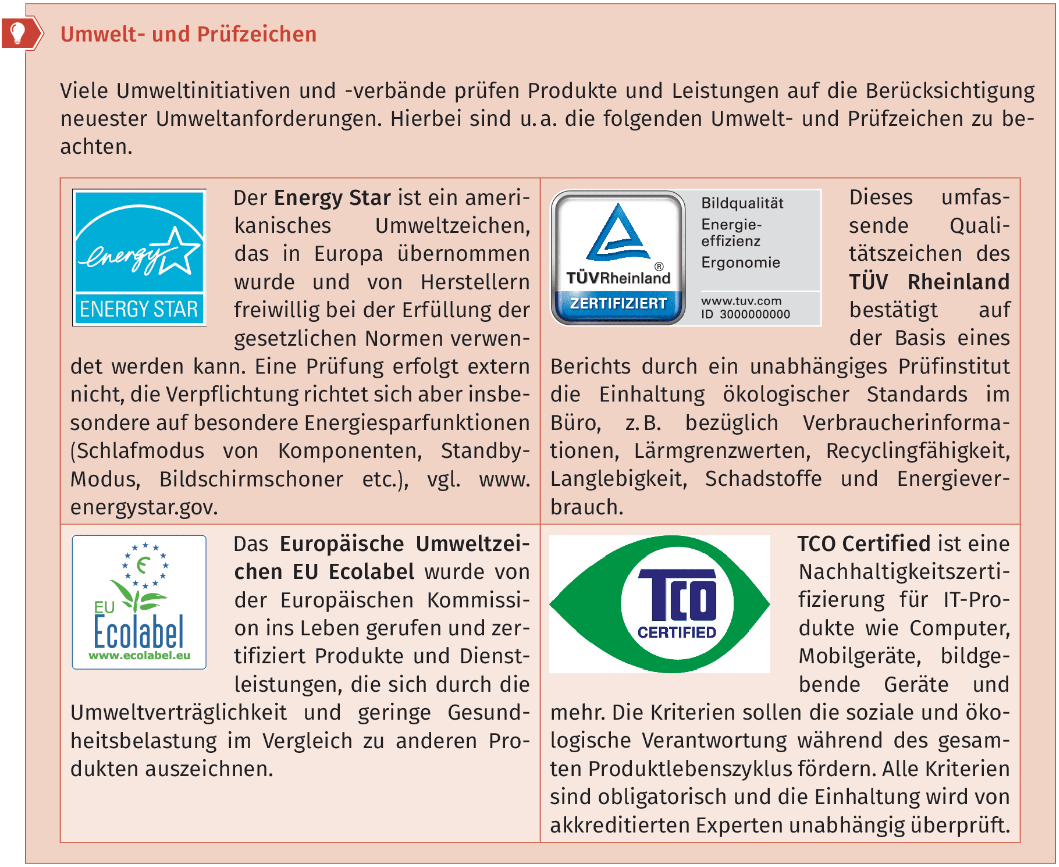
\includegraphics[width=0.7\textwidth]{./images/2.3.2_umweltzeichen.png}
        \caption{Umwelt- und Prüfzeichen}\label{fig:Umweltzeichen}
    \end{figure}

    \begin{tcolorbox}[width=11cm, center, title=Green-IT, coltitle=white, colframe=orange, colback=white!60!orange]
        Unternehmenskultur, IT möglichst umweltschonend zu beschaffen und einzusetzen.\\
        %TODO possible itemize here
        Umfang: Beschaffung, Nutzung, Verwertung und Entsorgung werden als Kreislauf angesehen. Ziel: möglichst wenig Ressourcenverbrauch \\
        Überprüfung: Erstellung von Nachhaltigkeitsrichtlinien, -konzepten, -berichten und -managmentsystemen
    \end{tcolorbox}

    \begin{tcolorbox}[width=14cm, center, title=Maßnahmenkatalog Green-IT, coltitle=white, colframe=orange, colback=white!60!orange]
        \begin{itemize}[itemsep=0.1em, parsep=0.3em]
            \item Bedarfsgerechter Einsatz von Hardware und Software prüfen
            \item Einsparung Energie und Energiekosten durch effiziente IT-Lösungen
            \item Beratung, den Lebenszyklus der Geräte zu verlängern, Kosten zu senken, Refurbished IT einzusetzen
            \item Bedarfsgerechter Betrieb der IT anstelle eines durchlaufenden Betriebs
            \item Energie und Kosten sparen durch Virtualisierung
            \item Einsatz umweltschonender Verbrauchsmaterialien
            \item Software auf Nachhaltigkeit prüfen, eventuell Open-Source-Software vorziehen
            \item Mitarbeiter auffordern, umweltfreundlich zu kommunizieren
        \end{itemize}
    \end{tcolorbox}

\subsection{Wirtschaftlichkeit von IT-Systemen erläutern}
    \begin{subindent}
        In Unternehmen muss wirtschaftlich gearbeitet werden. Hierfür ist bei allen Angeboten eine Wirtschaftslichkeitsbetrachtung durchzuführen, um das beste (nach den folgenden Punkten) zu finden.
    \end{subindent}

    \begin{tcolorbox}[width=11cm, center, title=Wirtschaftlichkeitsbetrachtungskriterien, coltitle=white, colframe=white!20!blue, colback=white!80!blue]
        \begin{itemize}[itemsep=0.01em, parsep=0.3em]
            \item Preisvergleiche
            \item Anschaffungs- und Zusatzkosten
            \item Folgekosten
            \item Restwerte
            \item Sonstige Kriterien (z.B. Lieferantenqualität)
        \end{itemize}
    \end{tcolorbox}

\subsection{IT-Sicherheit von IT-Systemen, Informations- und Datenschutz erläutern}
    \begin{subindent}
        \begin{itemize}[leftmargin=2.5cm, topsep=0.2em, itemsep=0.1em, parsep=0.3em]
            \item \textbf{Datenschutz} \\
                  Schutz privater, personenbezogener Daten eines jeden Menschen
            \item \textbf{Datensicherheit} \\
                  Schutz aller Daten in Unternehmen, unabhängig von Sachbezug oder Personenbezug
            \item \textbf{IT-Sicherheit} \\
                  Allgemeine Bezeichnung für Einsatz von Informationstechnik und den Schutz der damit verbundenen Anforderungen (s.\@ unten)
            \item \textbf{Informationssicherheit} \\
                  Schutz aller Informationen (digital/analog), genauere Eingrenzung durch BSI oder ISO 27001
        \end{itemize}
    \end{subindent}

    \begin{tcolorbox}[width=14cm, center, title=Gemeinsame Anforderungen für Daten und Systeme, coltitle=white, colframe=orange, colback=white!60!orange]
        \begin{itemize}[itemsep=0.1em, parsep=0.3em]
            \item \textbf{Vertraulichkeit:} nur für befugte Personen zugänglich
            \item \textbf{Integrität:} keine Verfälschung, Korrektheit
            \item \textbf{Verfügbarkeit:} Schutz vor Unterbrechungen/Ausfällen
        \end{itemize}
    \end{tcolorbox}
    %TODO S.148-149 Sicherheitsvorfälle und Maßnahmen maybe adden

\subsection*{Reflexion Kapitel 2.3}
\addcontentsline{toc}{subsection}{Reflexion Kapitel 2.3}
    \begin{refindent}
        Qualität und Leistungsfähigkeit werden durch verschieden Normen und Standards garantiert.
        Green-IT ist das Einsetzen von IT nach verschiedenen Nachhaltigkeitsideen/-konzepten.
        (Sehr) kurzer Anriss zu IT-Sicherheit und Maßnahmen dafür.
    \end{refindent}